\documentclass[12pt,a4paper]{article}

% Packages
\usepackage[utf8]{inputenc}
\usepackage[T1]{fontenc}
\usepackage{geometry}
\usepackage{graphicx}
\usepackage{hyperref}
\usepackage{enumitem}
\usepackage{xcolor}
\usepackage{tikz}
\usepackage{booktabs}
\usepackage{fancyhdr}
\usepackage{tcolorbox}
\usepackage{listings}
\usepackage{amsmath}
\usepackage{amssymb}
\usepackage{longtable}

% Page geometry
\geometry{margin=2.5cm}

% Colors
\definecolor{primaryblue}{RGB}{0, 102, 204}
\definecolor{successgreen}{RGB}{40, 167, 69}
\definecolor{dangerred}{RGB}{220, 53, 69}
\definecolor{warningyellow}{RGB}{255, 193, 7}
\definecolor{lightgray}{RGB}{248, 249, 250}
\definecolor{codegray}{RGB}{45, 45, 45}
\definecolor{codegreen}{RGB}{0, 128, 0}

% TikZ libraries
\usetikzlibrary{shapes, arrows, positioning, fit, backgrounds, calc, shapes.geometric}

% Listings setup
\lstset{
    basicstyle=\ttfamily\small,
    backgroundcolor=\color{lightgray},
    frame=single,
    framerule=0pt,
    breaklines=true,
    showstringspaces=false,
    keywordstyle=\color{primaryblue}\bfseries,
    commentstyle=\color{codegreen},
    stringstyle=\color{dangerred},
    numbers=left,
    numberstyle=\tiny\color{gray},
    numbersep=5pt,
    xleftmargin=15pt
}

% Header and footer
\pagestyle{fancy}
\fancyhf{}
\fancyhead[L]{\textbf{CS2113 -- Software Development Project}}
\fancyhead[R]{Lecture 5: Sprint 3}
\fancyfoot[C]{\thepage}

% Tcolorbox styles
\tcbuselibrary{skins, breakable, listings}

\newtcolorbox{keyinsight}{
    colback=primaryblue!10,
    colframe=primaryblue,
    title=\textbf{Key Insight},
    fonttitle=\bfseries,
    breakable
}

\newtcolorbox{warning}{
    colback=dangerred!10,
    colframe=dangerred,
    title=\textbf{Warning},
    fonttitle=\bfseries,
    breakable
}

\newtcolorbox{tip}{
    colback=successgreen!10,
    colframe=successgreen,
    title=\textbf{Tip},
    fonttitle=\bfseries,
    breakable
}

\newtcolorbox{definitionbox}{
    colback=lightgray,
    colframe=black!50,
    breakable
}

\newtcolorbox{commandbox}{
    colback=codegray!10,
    colframe=codegray,
    breakable
}

% Title
\title{
    \vspace{-1cm}
    \textbf{Sprint 3: Testing and Final Review}\\
    \large Lecture 5 Notes\\[0.5cm]
    \normalsize School of Computing Communication and Media Studies
}
\author{Masoud Hamad}
\date{CS2113 -- Software Development Project\\Academic Year 2025}

\begin{document}

\maketitle
\tableofcontents
\newpage

%============================================================
\section{Introduction to Sprint 3}
%============================================================

Sprint 3 is the final sprint of the course. Teams work on new user stories while focusing heavily on \textbf{testing practices}. Additionally, each team member must complete:

\begin{itemize}
    \item \textbf{Peer Review:} Assessing themselves and teammates
    \item \textbf{Final Report:} Individual reflection on the course
\end{itemize}

\begin{warning}
Both peer review and final report are \textbf{required to pass the course}. Submitting either after the Sprint deadline will decrease the personal grade.
\end{warning}

%============================================================
\section{Why Testing Matters}
%============================================================

\begin{definitionbox}
\textbf{Testing} ensures that code works as intended. Without automated tests, developers must manually verify all features after every change---an impractical approach at scale.
\end{definitionbox}

\subsection{The Problem: Regression Bugs}

\textbf{Regression bugs} occur when features that previously worked break after code changes. Manual testing becomes impractical because:

\begin{itemize}
    \item Every new feature requires re-testing all existing features
    \item Time required grows exponentially with project size
    \item Human testers make mistakes and miss edge cases
\end{itemize}

\subsection{The Solution: Automated Tests}

Automated tests:
\begin{itemize}
    \item Run quickly and consistently
    \item Catch regressions immediately
    \item Document expected behavior
    \item Enable confident refactoring
\end{itemize}

%============================================================
\section{The Test Pyramid}
%============================================================

Martin Fowler's Test Pyramid categorizes tests into three levels:

%------------------------------------------------------------
% Figure 1: Test Pyramid
%------------------------------------------------------------
\begin{figure}[htbp]
\centering
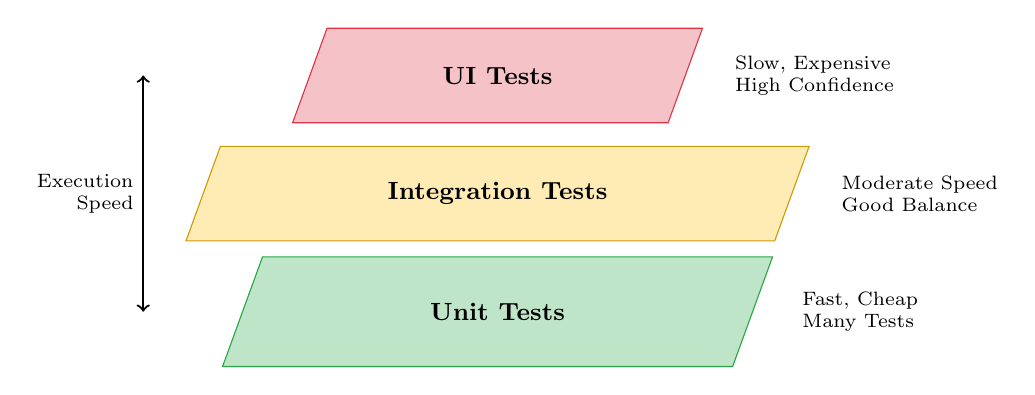
\begin{tikzpicture}[
    level/.style={trapezium, draw, trapezium left angle=70, trapezium right angle=110, minimum height=1.2cm, align=center, font=\small\bfseries}
]
    % UI Tests (top)
    \node[level, fill=dangerred!30, draw=dangerred, minimum width=3cm] (ui) at (0, 4) {UI Tests};

    % Integration Tests (middle)
    \node[level, fill=warningyellow!30, draw=warningyellow!80!black, minimum width=5cm] (int) at (0, 2.5) {Integration Tests};

    % Unit Tests (base)
    \node[level, fill=successgreen!30, draw=successgreen, minimum width=7cm] (unit) at (0, 1) {Unit Tests};

    % Labels on right
    \node[right=0.5cm, font=\scriptsize, align=left] at (ui.east) {Slow, Expensive\\High Confidence};
    \node[right=0.5cm, font=\scriptsize, align=left] at (int.east) {Moderate Speed\\Good Balance};
    \node[right=0.5cm, font=\scriptsize, align=left] at (unit.east) {Fast, Cheap\\Many Tests};

    % Arrow
    \draw[<->, thick] (-4.5, 1) -- (-4.5, 4);
    \node[left, font=\scriptsize, align=right] at (-4.5, 2.5) {Execution\\Speed};
\end{tikzpicture}
\caption{The Test Pyramid}
\label{fig:test-pyramid}
\end{figure}

\subsection{Trade-offs}

Moving up the pyramid:
\begin{itemize}
    \item \textcolor{successgreen}{\textbf{+}} Increases reliability/confidence
    \item \textcolor{dangerred}{\textbf{--}} Tests become harder to maintain
    \item \textcolor{dangerred}{\textbf{--}} Tests become slower to execute
    \item \textcolor{dangerred}{\textbf{--}} Tests become more expensive to implement
\end{itemize}

%============================================================
\section{Types of Tests}
%============================================================

\subsection{Unit Tests}

\begin{definitionbox}
\textbf{Unit Tests} test individual methods in isolation. They never integrate with other code parts like databases.
\end{definitionbox}

\begin{commandbox}
\begin{lstlisting}[language=Java]
@Test
void calculateWordsReturnsSingleWord() {
    String message = "Hello";
    assertEquals(1, MessageUtils.calculateWords(message));
}

@Test
void calculateWordsReturnsManyWords() {
    String message = "Hello world";
    assertEquals(2, MessageUtils.calculateWords(message));
}

@Test
void calculateWordsReturnsZeroForEmpty() {
    String message = "";
    assertEquals(0, MessageUtils.calculateWords(message));
}
\end{lstlisting}
\end{commandbox}

\textbf{Pros:}
\begin{itemize}
    \item Simple to implement and maintain
    \item Fast execution
\end{itemize}

\textbf{Cons:}
\begin{itemize}
    \item Limited reliability about overall application functionality
\end{itemize}

\subsection{Integration Tests}

\begin{definitionbox}
\textbf{Integration Tests} test that different application parts work together when integrated. Commonly test database operations and REST API endpoints.
\end{definitionbox}

\begin{keyinsight}
``Write tests. Not too many. Mostly integration.'' --- Guillermo Rauch, CEO of Vercel

Integration tests provide the best ``bang for your buck'' in confidence that applications work as intended.
\end{keyinsight}

\subsection{UI Tests (End-to-End)}

\begin{definitionbox}
\textbf{UI Tests} simulate real user interactions through the browser: navigating pages, filling forms, clicking buttons, verifying content.
\end{definitionbox}

\textbf{Pros:}
\begin{itemize}
    \item High reliability that application works end-to-end
\end{itemize}

\textbf{Cons:}
\begin{itemize}
    \item Difficult to implement
    \item Laborious to maintain
    \item Slow execution time
\end{itemize}

%============================================================
\section{Testing REST API Endpoints}
%============================================================

\subsection{Test Class Structure}

\begin{commandbox}
\begin{lstlisting}[language=Java]
@SpringBootTest
@AutoConfigureMockMvc
public class QuizRestControllerTest {

    @Autowired
    private QuizRepository quizRepository;

    @Autowired
    private MockMvc mockMvc;

    private ObjectMapper mapper = new ObjectMapper();

    @BeforeEach
    void setUp() {
        quizRepository.deleteAll();
    }
}
\end{lstlisting}
\end{commandbox}

\subsection{Key Annotations}

\begin{itemize}
    \item \texttt{@SpringBootTest} -- Loads Spring context for tests
    \item \texttt{@AutoConfigureMockMvc} -- Enables MockMvc injection
    \item \texttt{@BeforeEach} -- Runs before each test (clean database)
    \item \texttt{@Test} -- Marks a test method
\end{itemize}

\subsection{Test Independence}

\begin{warning}
Each test should start with an \textbf{empty database} to ensure test independence. Tests should not depend on other tests' data or execution order.
\end{warning}

%============================================================
\section{Arrange-Act-Assert Pattern}
%============================================================

Structure each test in three phases:

%------------------------------------------------------------
% Figure 2: AAA Pattern
%------------------------------------------------------------
\begin{figure}[htbp]
\centering
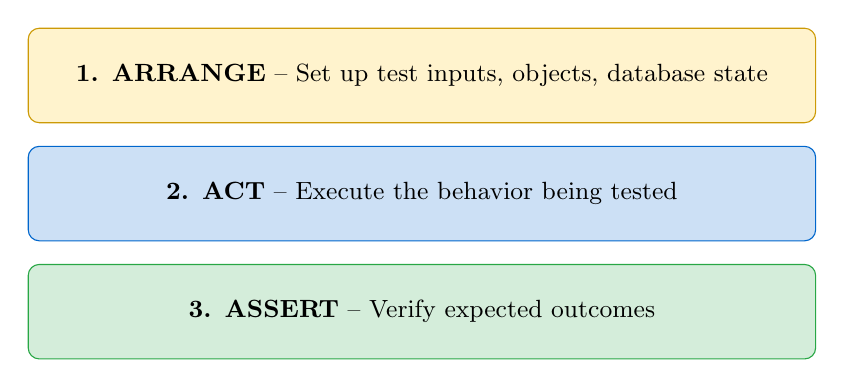
\begin{tikzpicture}[
    node distance=0.5cm,
    phase/.style={rectangle, draw=primaryblue, fill=primaryblue!10, rounded corners, minimum width=10cm, minimum height=1.2cm, align=left, font=\small}
]
    \node[phase, fill=warningyellow!20, draw=warningyellow!80!black] (arrange) at (0, 2) {\textbf{1. ARRANGE} -- Set up test inputs, objects, database state};
    \node[phase, fill=primaryblue!20] (act) at (0, 0.5) {\textbf{2. ACT} -- Execute the behavior being tested};
    \node[phase, fill=successgreen!20, draw=successgreen] (assert) at (0, -1) {\textbf{3. ASSERT} -- Verify expected outcomes};
\end{tikzpicture}
\caption{Arrange-Act-Assert Pattern}
\label{fig:aaa-pattern}
\end{figure}

%============================================================
\section{GET Request Tests}
%============================================================

\begin{commandbox}
\begin{lstlisting}[language=Java]
@Test
public void getAllQuizzesReturnsEmptyList() throws Exception {
    // Act & Assert
    this.mockMvc.perform(get("/api/quizzes"))
        .andExpect(status().isOk())
        .andExpect(jsonPath("$", hasSize(0)));
}

@Test
public void getQuizByIdReturnsQuiz() throws Exception {
    // Arrange
    Quiz quiz = new Quiz("Test Quiz", "Description");
    quizRepository.save(quiz);

    // Act & Assert
    this.mockMvc.perform(get("/api/quizzes/" + quiz.getId()))
        .andExpect(status().isOk())
        .andExpect(jsonPath("$.name").value("Test Quiz"))
        .andExpect(jsonPath("$.id").value(quiz.getId()));
}

@Test
public void getQuizByIdReturnsNotFound() throws Exception {
    // Act & Assert
    this.mockMvc.perform(get("/api/quizzes/999"))
        .andExpect(status().isNotFound());
}
\end{lstlisting}
\end{commandbox}

%============================================================
\section{POST Request Tests}
%============================================================

\begin{commandbox}
\begin{lstlisting}[language=Java]
@Test
public void createQuizSavesValidQuiz() throws Exception {
    // Arrange
    CreateQuizDto quiz = new CreateQuizDto("New Quiz");
    String requestBody = mapper.writeValueAsString(quiz);

    // Act
    this.mockMvc.perform(post("/api/quizzes")
            .contentType(MediaType.APPLICATION_JSON)
            .content(requestBody))
        // Assert
        .andExpect(status().isOk())
        .andExpect(jsonPath("$.name").value("New Quiz"));

    // Verify database
    List<Quiz> quizzes = quizRepository.findAll();
    assertEquals(1, quizzes.size());
    assertEquals("New Quiz", quizzes.get(0).getName());
}

@Test
public void createQuizRejectInvalidQuiz() throws Exception {
    // Arrange
    CreateQuizDto quiz = new CreateQuizDto(""); // Empty name
    String requestBody = mapper.writeValueAsString(quiz);

    // Act & Assert
    this.mockMvc.perform(post("/api/quizzes")
            .contentType(MediaType.APPLICATION_JSON)
            .content(requestBody))
        .andExpect(status().isBadRequest());

    // Verify nothing saved
    assertEquals(0, quizRepository.findAll().size());
}
\end{lstlisting}
\end{commandbox}

%============================================================
\section{Test Configuration}
%============================================================

\subsection{Separate Test Database}

Create \texttt{src/test/resources/application.properties}:

\begin{commandbox}
\begin{lstlisting}
spring.datasource.url=jdbc:h2:mem:quizzer-test;DB_CLOSE_ON_EXIT=FALSE
spring.jpa.hibernate.ddl-auto=create-drop
\end{lstlisting}
\end{commandbox}

\subsection{Required Dependencies}

\begin{commandbox}
\begin{lstlisting}[language=XML]
<dependency>
    <groupId>org.springframework.boot</groupId>
    <artifactId>spring-boot-starter-test</artifactId>
    <scope>test</scope>
</dependency>

<dependency>
    <groupId>com.jayway.jsonpath</groupId>
    <artifactId>json-path</artifactId>
    <version>2.8.0</version>
    <scope>test</scope>
</dependency>
\end{lstlisting}
\end{commandbox}

\subsection{Running Tests}

\begin{commandbox}
\begin{lstlisting}[language=bash]
# Run all tests
./mvnw test

# Run specific test class
./mvnw test -Dtest=QuizRestControllerTest

# Run with verbose output
./mvnw test -X
\end{lstlisting}
\end{commandbox}

%============================================================
\section{Test Naming Conventions}
%============================================================

Use descriptive names that explain:
\begin{itemize}
    \item What is being tested
    \item Under what conditions
    \item Expected outcome
\end{itemize}

\textbf{Good Examples:}
\begin{itemize}
    \item \texttt{getAllQuizzesReturnsEmptyListWhenNoQuizzesExist}
    \item \texttt{getQuizByIdReturnsNotFoundWhenQuizDoesNotExist}
    \item \texttt{createAnswerDoesNotSaveForUnpublishedQuiz}
\end{itemize}

%============================================================
\section{Peer Review}
%============================================================

\begin{definitionbox}
\textbf{Peer Review} assesses each team member's contributions. Personal grades derive from peer reviews and teacher observations.
\end{definitionbox}

\subsection{Evaluation Criteria}

Each team member is graded (0--5) on:

\begin{enumerate}
    \item \textbf{Activity in Team Work}
    \begin{itemize}
        \item Meeting attendance
        \item Active presence and engagement
        \item Communication outside meetings
    \end{itemize}

    \item \textbf{Technical Contributions}
    \begin{itemize}
        \item Amount of working code written
        \item Active participation in coding (pair programming)
        \item Code quality
    \end{itemize}

    \item \textbf{Project Management \& Documentation}
    \begin{itemize}
        \item Backlog management
        \item Process improvement (retrospectives)
        \item Documentation writing
    \end{itemize}
\end{enumerate}

\begin{tip}
Peer reviews are \textbf{anonymous}---team members don't see each other's reviews. Be honest and constructive!
\end{tip}

%============================================================
\section{Final Report}
%============================================================

The final report answers five questions:

\subsection{Question 1: Scrum Events}
\begin{itemize}
    \item List the four Scrum events during a Sprint
    \item Describe the purpose of each event
    \item Assess your team's success in fulfilling each event's purpose
\end{itemize}

\subsection{Question 2: Team Assessment}
\begin{itemize}
    \item Identify areas where your team succeeded
    \item Identify areas needing improvement
\end{itemize}

\subsection{Question 3: Personal Assessment}
\begin{itemize}
    \item Identify your personal strengths
    \item Identify areas for personal improvement
\end{itemize}

\subsection{Question 4: Advice for New Teams}
\begin{itemize}
    \item Provide three important recommendations
    \item Justify based on your course experiences
\end{itemize}

\subsection{Question 5: Learning Reflection}
\begin{itemize}
    \item Describe what you learned during the course
    \item Identify topics for deeper exploration
\end{itemize}

%============================================================
\section{Final Checklist}
%============================================================

%------------------------------------------------------------
% Figure 3: Final Checklist
%------------------------------------------------------------
\begin{figure}[htbp]
\centering
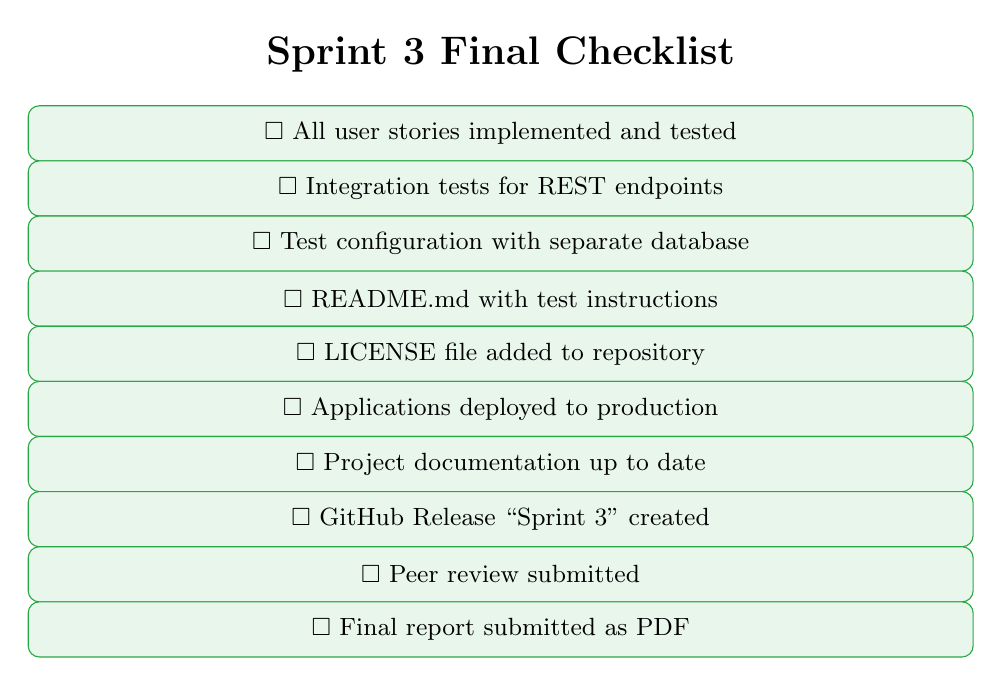
\begin{tikzpicture}[
    node distance=0.4cm,
    item/.style={rectangle, draw=successgreen, fill=successgreen!10, rounded corners, minimum width=12cm, minimum height=0.7cm, align=left, font=\small}
]
    \node[font=\Large\bfseries] at (0, 5) {Sprint 3 Final Checklist};

    \node[item] at (0, 4) {$\square$ All user stories implemented and tested};
    \node[item] at (0, 3.3) {$\square$ Integration tests for REST endpoints};
    \node[item] at (0, 2.6) {$\square$ Test configuration with separate database};
    \node[item] at (0, 1.9) {$\square$ README.md with test instructions};
    \node[item] at (0, 1.2) {$\square$ LICENSE file added to repository};
    \node[item] at (0, 0.5) {$\square$ Applications deployed to production};
    \node[item] at (0, -0.2) {$\square$ Project documentation up to date};
    \node[item] at (0, -0.9) {$\square$ GitHub Release ``Sprint 3'' created};
    \node[item] at (0, -1.6) {$\square$ Peer review submitted};
    \node[item] at (0, -2.3) {$\square$ Final report submitted as PDF};
\end{tikzpicture}
\caption{Sprint 3 Final Checklist}
\label{fig:checklist}
\end{figure}

%============================================================
\newpage
\section{Exercises}
%============================================================

\begin{tcolorbox}[colback=warningyellow!10, colframe=warningyellow!80!black, title=\textbf{Sprint 3 Deadline}]
All work must be pushed to GitHub repository before the final deadline. Peer review and final report are \textbf{required to pass}.
\end{tcolorbox}

\subsection{Exercise 1: Retrospective}
Conduct a Mad-Sad-Glad retrospective for Sprint 2. Compare with Sprint 1 retrospective to identify recurring issues.

\subsection{Exercise 2: Select Scrum Master}
Choose a new Scrum Master for Sprint 3 (different from Sprint 2).

\subsection{Exercise 3: Close Sprint 2 Issues}
Close completed Sprint 2 issues and create Sprint 3 milestone.

\subsection{Exercise 4: Create User Story Issues}
Create issues for Sprint 3 user stories (Review feature).

\subsection{Exercises 5--8: Task Planning}
Break down each Sprint 3 user story into technical tasks.

\subsection{Exercise 9: Test Configuration}
Add test-specific configuration file with separate database.

\subsection{Exercise 10: Test All Quizzes Endpoint}
Implement tests:
\begin{itemize}
    \item Returns empty list when no quizzes exist
    \item Returns list when published quizzes exist
    \item Does not return unpublished quizzes
\end{itemize}

\subsection{Exercise 11: Test Quiz Questions Endpoint}
Implement tests:
\begin{itemize}
    \item Returns empty list when quiz has no questions
    \item Returns list with questions and answer options
    \item Returns error when quiz doesn't exist
\end{itemize}

\subsection{Exercise 12: Test Create Answer Endpoint}
Implement tests:
\begin{itemize}
    \item Saves answer for published quiz
    \item Rejects answer without answer option
    \item Rejects answer for non-existing option
    \item Rejects answer for unpublished quiz
\end{itemize}

\subsection{Exercise 13: Additional Endpoint Tests}
Implement tests for at least two additional endpoints of your choice.

\subsection{Exercise 14: Update Documentation}
Add test running instructions to README.md Developer Guide.

\subsection{Exercise 15: Add License}
\begin{itemize}
    \item Choose a license (MIT recommended)
    \item Create LICENSE file in repository root
    \item Add license info to README.md
\end{itemize}

\subsection{Exercise 16: Deploy Applications}
Deploy final versions of backend and frontend to production.

\subsection{Exercise 17: Update Project Documentation}
Ensure all documentation is current:
\begin{itemize}
    \item Project description
    \item Data model
    \item Developer guide
    \item Swagger documentation
\end{itemize}

\subsection{Exercise 18: Create Release}
Create GitHub release ``Sprint 3'' with feature description.

\subsection{Exercise 19: Peer Review}
Complete peer review for all team members including yourself.

\subsection{Exercise 20: Final Report}
Write and submit final report answering all five questions as PDF.

%============================================================
\vspace{1cm}
\hrule
\vspace{0.3cm}
\begin{center}
\small
\textit{This document is licensed under Creative Commons BY-NC-SA 4.0}
\end{center}

\end{document}
